\chapter{On Excitability and How to Model It}
\label{excitab} % Always give a unique label
\chaptermark{Excitability}


\abstract{This chapter presents the basic principles of cell excitability, under the perspective of how it may be described and explored with models. I will be mostly referring to the generation of \textit{action potentials},which are electrical pulses that travel along the membrane of cells in the nervous system, muscles, heart, and the endocrine system. The way these pulses ignite, propagate through space, and are transformed into chemical signals is a fascinating outcome of natural evolution, emerging as an effective rapid mean of communication across cells and tissues, as well as at the subcellular level.}

\vspace{2cm} % Adds 1 centimeter of vertical space

\begin{svgraybox}
{\bf{Learning objectives}}
\begin{itemize}
	\item This is the first item.
	\item This is the second item.
	\item You can add as many items as you need.
	\item Here's another item.
  \end{itemize}
\end{svgraybox}

\clearpage

\section{Introduction}\label{sec3:1}
To be written\dots


\begin{figure}[t]
	\sidecaption[t]
	\centering
	\includegraphics[scale=1.5]{Hodgkin_Huxley.jpg}
	%\picplace{5cm}{2cm} % Give the correct figure height and width in cm
	\caption{Alan Hodgkin (1914--98) and Huxley (1917--2012).}\label{fig3:HodgkinHuxley}       % Give a unique label
	\end{figure}

\section{Going beyond the passive membranes bottlenecks}

\subsection{The conservation of charge: old principles and new insights}

\subsection{Temporal Integration}

\subsection{Nobel-prize winning intuitions: active and passive ionic permeability}

\subsection{Mass-action law and chemical reactions}
\subsection{Opening and closing of ion channels in the language of kinetic schemes}




\section{The Conductance Based Models for biophysical accuracy}\label{sec3:2}
\subsection{The Hodgkin Huxley Model: a 60 years old milestone for the field}
\subsection{Morris-Lecar: a balance between biophysical plausibility and tractability}
\subsection{On the intrinsic variability of spike timing}
\subsection{Ion channels flickering and a first encounter with noise in neural systems}

\section{Integrate-and-Fire excitability: early insights and modern significance}\label{sec3:3}

\subsection{``As simple as possible, but not simpler''}
This title is a portion of a famous quote, by Albert Einstein that sticked with me over the years. It is of course not trivial to understand what is the level of simplicity to adopt, in the description of (bio)physical phenomena. I have also been fascinated by the insights of the philosophers (of Science) as Karl Popper. I found remarkable his recommendation for any scientific theory: it must be easily \textit{falsifiable} for it  to have higher chances to be correct. Today this very concept is in the DNA of researchers across many disciplines. Popper exemplified his point criticizing Astrology, for its large number and variety of presumed \textit{zodiacal} influences that make it likely to account \textit{a posteriori} for almost any outcome of human daily life events. However, the very same inherent complications and richness of details and features makes it very hard to identify a scenario to challenge Astrology's predictions! In other words, Astrology is not \textit{simple} at all.

A similar feeling is commonly embraced by physicists, who almost always first initiate a theoretical inquiries with a minimal description and with the simplest possible scenario of a system under consideration. Also data scientists and statisticians have clear in mind the very same concept, and rephrase it in terms of avoiding \textit{overfitting} a model to certain observations or dataset, due to an excessively large number of degrees of freedom when reproducing a dataset. If this happens, it is unlikely that the model will generalize to data it was never trained on.


In Computational Neuroscience, we should then always be mindful when adopting a very complicated description of a biophysical phenomenon, and when a very large number of parameters is a critical requirement of a model, even beyond the feasibility of their actual identification from experiments. Hopefully, we should make our models as simple as possible, and we should set the condition for its predictions to be falsified: that is when we learn, in a virtuous interaction between experiments and theory.

\begin{figure}[t]
	\sidecaption[t]
	\centering
	\includegraphics[scale=.75]{Popper_Einstein_Lapique.jpg}
	%\picplace{5cm}{2cm} % Give the correct figure height and width in cm
	\caption{Karl Popper (1902--94), Albert Einstein (1879--1955), and Louis Lapique (1866--1952)}
	\label{fig3:PopperEinsteinLapique}       % Give a unique label
	\end{figure}



There is however another important consideration I would like to present. This originally escaped my own appreciation as a young student. At that time, after learning about Hodgkin and Huxley's seminal work, I did feel empowered to imagine its arbitrary extension \textit{in principle}: any number of additional ionic currents could be included using Markov kinetic schemes, a more accurate description of cell's morphology could always be captured by cable theory, and electrodiffusion for a variety of ionic concentrations could be easily coupled with all the other equations, to name a few. As computers were used to solve the model equations and perform numerical simulations, I thought that only the sky was the limit. My optimism was perhaps only partly correct. As for weather forecasts, I imagined that large scale supercomputers could \textit{crunch numbers} and solve a huge number of equations, describing any complex (weather) model, and ultimately produce predictions for (atmospheric) physical variables in the immediate and near future. However, even assuming that all the equations and parameters and are known and do capture correctly the underlying physical reality, two problems remain: 1) \textit{number crunching} alone requires time to be completed, sometimes a substantial amount of time; 2) simulating a model on a digital computer requires iteratively feeding partial numerical results into a series of mathematical expressions, and numerical errors may accumulate. Both issues come as computers are intrinsically discrete \textit{in time} and limited in their numerical resolution, so that rounding errors or imperfect numerical processing might decrease our confidence over model behavior as the simulated time goes by. I am also hinting at the possible sensitivity of the model, sometimes called \textit{robustness}, to the precise representation of its parameters or combination of parameters and initial conditions. 

In my humber opinion, these become serious issues, as the the intuition and insights that a computational neuroscientist gains through time, when developing, testing, and exploring their model might be challenged. In fact, the time one has to wait for a simulation to complete does unavoidably makes it harder for a deep intuition to develop on how, e.g., changing one parameter affects the subtle behavior of a certain phenomenon. 

As a final central point, rich and complicated models might further make it hard for the scientist to recognize invariants or identify key mechanisms and principles, as they ultimately are hardly mathematical tractable, in terms of derivation of general results.

\begin{figure}[t]
\sidecaption[t]
\centering
\includegraphics[scale=.33]{A}
%\picplace{5cm}{2cm} % Give the correct figure height and width in cm
\caption{Please write your figure caption here}
\label{fig3:A1}       % Give a unique label
\end{figure}



\subsection{From conductance-based to Integrate-and-Fire models}

Those who are mathematically inclined, may appreciate a very early elegant presentation, by Larry Abbott and Kepler (??), deriving integrate-and-fire models equations from conductance-based descriptions. On a first approximation, you are separating time scales associated to the many state variable of a neuron model. Focusing for instance only on the role of ionic conductances contributing to the initiation of an action potential, a similar procedure rewrites the charge-balance equation.

\subsection{The linear Integrate-and-Fire model}

When considering neuronal activation, some variables operate much faster than others, potentially reaching a steady state instantaneously. Take, for example, the 'm' variable and its associated function, 'm infinity,' which represents this asymptotic state. One could simplify the model by focusing solely on this rapid activation and using fewer parameters to describe action potential initiation. However, such a simplified model might fail to capture the complexities of neuronal activity, particularly the spatial dynamics of signal conduction.

A more practical approach to defining 'integrate-and-fire' neurons stems from recognizing that the action potential itself is a highly stereotyped event. Its amplitude carries little information; therefore, as a first approximation, it's reasonable to conserve computational resources and avoid detailed analysis of the action potential's exact trajectory. This perspective leads to a simplified model with only two main variables: the membrane potential and the integrated input current. This simplification is particularly relevant for cortical neurons, which exhibit sparse activity, firing action potentials only briefly before returning to a resting state. Consequently, we can describe the membrane potential's evolution up to the point of action potential firing and then resume the description after the action potential concludes.

\begin{figure}[t]
\sidecaption[t]
\centering
\includegraphics[scale=.33]{B}
%\picplace{5cm}{2cm} % Give the correct figure height and width in cm
\caption{Please write your figure caption here}
\label{fig3:A2}       % Give a unique label
\end{figure}


Several approaches exist to describe the equation governing this simplified model. The simplest, known as the 'linear integrate-and-fire with threshold' model, treats the neuron as a perfect integrator. The membrane potential's derivative is directly proportional to the input current. This simplification disregards the subthreshold influence of individual voltage-gated ion channels, which contribute to neuronal integration. However, for exploratory purposes, focusing on this simplified phenomenon can be valuable.

It's important to highlight that this model adopts a 'point neuron' perspective. Most integrate-and-fire models aim to describe the electrical activity of neurons as a single point unit, effectively ignoring the complexities of dendritic integration. This simplification can be considered a temporary measure, with the complexities of dendritic processing potentially addressed in more advanced models.

By accepting this point neuron approximation, we can describe the electrical behavior of a neuron using a limited number of state variables, typically just the membrane potential, which varies over time without spatial considerations. However, it's crucial to acknowledge that this perfect integrator model has limitations. It doesn't accurately reflect the membrane potential's response to inhibitory and excitatory inputs, as it would unrealistically accumulate charge without returning to the resting membrane potential.


Let's add a constant parameter, potentially a negative number, to the right-hand side of our equation. This introduces a balance between the input strength and a 'pulling force' that determines the decay rate of the membrane potential. Consequently, the membrane potential avoids indefinite accumulation and instead decays towards a resting value in the absence of synaptic input.

However, without any constraints, the membrane potential could theoretically approach negative infinity. To prevent this, especially when synaptic activity isn't consistently excitatory, we introduce a lower boundary or 'floor.' This acts as a clipping mechanism, preventing the membrane potential from decreasing beyond a certain hyperpolarized value.

With this addition, our model's equation becomes: dV/dt = -beta + I<sub>ext</sub>, where 'beta' represents the decay rate and I<sub>ext</sub> represents the external current, which could be synaptic in nature. This simple model highlights the interplay between capacitance, decay rate, and threshold in shaping neuronal integration.

While this model doesn't fully capture the complexities of real neurons, its simplicity offers valuable insights. For instance, we can explore the concept of a fixed action potential threshold. Although a precise threshold isn't feasible in real neurons or even in detailed conductance-based models, assuming a fixed threshold allows us to define a firing mechanism for our model.

When the membrane potential exceeds this threshold, the neuron is said to have fired an action potential, and the membrane potential is instantly reset to a lower value. This reset value, typically above the resting potential, can reflect the after-spike hyperpolarization observed in real neurons.

Furthermore, we can incorporate a refractory period, a brief period following an action potential where the neuron cannot integrate new inputs. This phenomenologically captures the transient inactivation of ion channels observed in real neurons.

This simple model allows us to derive analytical relationships between input current and output firing frequency. By considering the absolute refractory period, we can even determine a maximum firing frequency, an upper bound that wouldn't be easily attainable with more complex models.

Analyzing the f-I curve, a plot of firing frequency versus input current, is a standard experimental protocol for characterizing neuron types. In our model, a negative current results in no spikes, as the membrane potential continuously decreases until it reaches the lower boundary.

For spiking to occur, the input current must exceed a minimal value known as the rheobase. If the current equals the decay rate (beta), the membrane potential remains constant. When the current surpasses beta, the membrane potential increases and eventually reaches the threshold.

By solving the differential equation, we can calculate the time it takes for the membrane potential to reach the threshold from a given starting point. This interspike interval is constant under constant input, matching the behavior of some real neurons and allowing us to calculate the average firing frequency.

Despite its simplicity, this model provides insights into the roles of capacitance and decay in neuronal firing. We can even extend the model to consider random, Poisson-distributed input arrival times, simulating fluctuating synaptic inputs. This leads to a stochastic process for the membrane potential, offering a simplified description of certain neuronal regimes.


In these lectures, we'll simplify the complexities of neuronal excitability we've discussed in previous weeks. Last week, we explored the Hodgkin-Huxley model, which uses the charge balance equation to describe neuronal dynamics. This model incorporates various ion channels, such as sodium and potassium channels, and their associated conductances and gating variables. These variables, like 'm' and 'h' in the Hodgkin-Huxley model, influence the flow of ions across the membrane, shaping the action potential.

Today, we'll focus on a simpler model called the integrate-and-fire model. This model capitalizes on the stereotypical nature of action potentials, simplifying the complex dynamics of ion channels. While the Hodgkin-Huxley model requires computationally intensive simulations, the integrate-and-fire model allows for more efficient simulations and even pen-and-paper calculations.

One key aspect we'll explore is the relationship between input current and firing frequency, represented by the f-I curve. This curve illustrates how a neuron's firing rate changes in response to varying input currents. With the integrate-and-fire model, we can derive an analytical expression for the f-I curve, providing insights into neuronal behavior without relying on complex simulations.

To begin, let's revisit the passive membrane properties. We'll simplify the neuron to an RC circuit, where 'R' represents the membrane resistance and 'C' represents the membrane capacitance. This simplification disregards the complexities of voltage-gated ion channels, focusing solely on the passive flow of current across the membrane.

In the integrate-and-fire model, we introduce a fixed threshold. When the membrane potential reaches this threshold, we say the neuron has fired an action potential. This simplification disregards the intricate dynamics of ion channel activation and inactivation that shape the action potential in real neurons.

After firing, the membrane potential is instantly reset to a lower value and held there for a brief refractory period. This mimics the refractory period observed in real neurons, where they are temporarily unable to fire another action potential.

This simplified model, with its fixed threshold and reset mechanism, allows us to explore neuronal behavior under different input conditions. We can analyze how the membrane potential integrates input current and how the firing frequency changes with varying input strengths.

To make the model more realistic, we can incorporate additional features, such as adaptation. This reflects the phenomenon observed in real neurons where their firing rate decreases over time in response to a constant input. We can achieve this by adding an adaptation current that acts as a negative feedback mechanism, reducing the firing frequency as the neuron becomes more active.

One way to understand adaptation is by considering the role of calcium ions. During an action potential, calcium ions flow into the neuron, and their concentration increases. This increase can activate calcium-dependent ion channels, which in turn can hyperpolarize the neuron, reducing its excitability and firing rate.

By incorporating calcium dynamics into the integrate-and-fire model, we can capture the phenomenon of spike frequency adaptation. This allows the model to more accurately reflect the behavior of real neurons, which exhibit a decrease in firing rate over time in response to a constant input.

While the integrate-and-fire model is a simplification, it offers valuable insights into neuronal behavior. It allows us to explore fundamental principles of neuronal integration and firing, and it can be extended to incorporate additional complexities, such as adaptation and calcium dynamics. By understanding the strengths and limitations of this model, we can gain a deeper appreciation for the intricate workings of real neurons and their role in shaping brain function.

To illustrate the usefulness of the integrate-and-fire model, let's examine some experimental data. We'll compare the f-I curves of real neurons with those predicted by the model. In these experiments, we recorded from different types of neurons in the somatosensory cortex of rats, including pyramidal cells and interneurons.

By injecting varying levels of current into these neurons, we observed how their firing rates changed. We then compared these experimental f-I curves with those generated by the integrate-and-fire model, adjusting the model parameters to best fit the data.

The results showed a remarkable agreement between the experimental and model-generated f-I curves. This suggests that the integrate-and-fire model, despite its simplicity, can effectively capture the firing behavior of real neurons. This is particularly valuable because it allows us to explore neuronal dynamics without resorting to complex and computationally expensive models like the Hodgkin-Huxley model.

However, it's important to acknowledge the limitations of the integrate-and-fire model. One key limitation is its inability to accurately predict the precise timing of action potentials. This is because the model's fixed threshold mechanism doesn't fully capture the dynamic interplay of ion channels that shape the action potential in real neurons.

To address this limitation, alternative models have been developed, such as the exponential integrate-and-fire model. This model incorporates a more realistic threshold mechanism that accounts for the explosive activation of sodium channels near the threshold. By doing so, it can more accurately predict the timing of action potentials, especially in response to fluctuating inputs.

The integrate-and-fire model, despite its limitations, remains a valuable tool in neuroscience research. Its simplicity allows for efficient simulations and analytical calculations, providing insights into neuronal behavior and network dynamics. By understanding its strengths and limitations, we can effectively utilize this model to explore the complexities of brain function and develop a deeper appreciation for the intricate workings of neurons.

In addition to its applications in single neuron modeling, the integrate-and-fire model can also be extended to simulate networks of interconnected neurons. This allows us to explore how populations of neurons interact and generate complex dynamics, offering insights into network-level phenomena such as oscillations and synchronization.

Imagine a network of integrate-and-fire neurons connected by synapses. When a neuron fires an action potential, it sends a signal to its downstream synaptic partners. This signal can either excite or inhibit the partner neuron, influencing its likelihood of firing.

By simulating such networks, we can investigate how different connectivity patterns and synaptic properties shape network activity. This can help us understand how the brain processes information and generates complex behaviors.

Furthermore, the integrate-and-fire model can be adapted to incorporate various levels of realism. For instance, we can include different types of neurons with distinct firing properties, or we can model the spatial structure of neurons, considering the dendritic and axonal compartments.

These extensions allow us to explore a wider range of neuronal phenomena and network dynamics. For example, we can investigate how different neuron types contribute to network oscillations, or how dendritic integration influences neuronal firing.

Overall, the integrate-and-fire model provides a versatile framework for exploring neuronal and network dynamics. Its simplicity allows for efficient simulations and analytical calculations, while its flexibility enables the incorporation of various levels of realism. By utilizing this model effectively, we can gain a deeper understanding of the brain's intricate workings and unravel the complexities of neural information processing.

It's important to remember that the integrate-and-fire model, while a powerful tool, is still a simplification of real neuronal behavior. It captures essential features of neuronal dynamics, but it disregards many intricate details.

For instance, the model assumes a fixed threshold for action potential generation, whereas real neurons exhibit more complex threshold dynamics due to the interplay of various ion channels. Additionally, the model typically represents neurons as point units, neglecting their spatial structure and the complexities of dendritic integration.

Despite these simplifications, the integrate-and-fire model has proven remarkably successful in capturing a wide range of neuronal phenomena. It has been used to study single neuron behavior, network dynamics, and even cognitive processes.

Moreover, the model's simplicity allows for analytical tractability, enabling the derivation of mathematical relationships that provide insights into neuronal function. This analytical tractability is a major advantage over more complex models, which often require computationally intensive simulations.

As we conclude our exploration of the integrate-and-fire model, it's crucial to recognize that it represents just one member of a broader family of simplified neuron models. Each model within this family offers a unique balance between simplicity and biological realism.

For instance, some models emphasize mathematical tractability, allowing for analytical solutions and insights into fundamental principles. Others prioritize biological accuracy, incorporating more detailed representations of ion channels and dendritic integration.

The choice of which model to use depends on the specific research question and the desired level of detail. For studies focused on network dynamics, a simpler model like the integrate-and-fire model might suffice. However, for investigations into the intricate dynamics of single neurons, a more detailed model might be necessary.

Researchers are continually developing new and improved neuron models, striving to strike an optimal balance between simplicity and realism. These models are essential tools for understanding the complexities of brain function and unraveling the mysteries of neural information processing.


\section{Bestiary of Integrate-and-Fire models: take your pick}
\subsection{The non-linear Integrate-and-Fire models: quadratic and exponential}
\subsection{Reverse engineering the IF model parameters from experimental data}
\subsection{The McCullogh-Pitts’ models: an extreme yet rewarding slimming cure}


\section{Multi-compartmental models and the relevance of morphology}
\subsection{Cable Theory and Rall’s model}

\section{How to link the dynamics of ionic concentrations into electrical models}

\section{Which model to use? The choice of model depends on level of analysis}

\newpage
\begin{svgraybox}
	{\bf{The Dirac's delta function: \(\delta(x)\)}}
	\\

	\(\delta(x)\) is due to the physicist Paul Dirac and, since its first use in 1930 for Quantum Mechanics, it found many applications in fields as diverse as Engineering and Statistics. It represents an \textit{impulse}: a sudden and extreme increase in the value of some quantity. Think of it as a huge spike, yet restricted to a tiny spot in space or in time. It is also used to express initial conditions or concentrations, when restricted to a sharp position in space or time. Beware! It stretches the concept of regular functions, as \(\sin(x), \ln(x), \cdots \), and it belong to the family of generalized  functions, called \textit{distributions}. An intuitive grasp of \(\delta(x)\) comes from its graph: it is \textit{zero} everywhere over the \(x\)-axis, except at \(x =0\) where it takes an infinite positive value.

	\begin{tikzpicture}
	\begin{scope}
	% Draw the axes
	\draw[->] (-2,0) -- (2,0) node[right] {$x$};
	\draw[->] (0,-0.5) -- (0,1.5) node[right] {$\delta(x)$};
  
	% Draw the Dirac delta function (centered)
	\draw[->, ultra thick] (0,0) -- (-0,1);
  
	% Add 0 to the origin
	\node[below right] at (0,0) {0};
	\end{scope}

	\begin{scope}[shift={(5,0)}] % Adjust (5,0) to change the spacing
	% Draw the axes
	\draw[->] (-2,0) -- (2,0) node[right] {$x$};
	\draw[->] (0,-0.5) -- (0,1.5) node[right] {$\delta(x-1)$};
  
	% Draw the Dirac delta function (centered)
	\draw[->, ultra thick] (1,0) -- (1,1);
  
	% Add 0 to the origin
	\node[below] at (1,0) {1};
	\end{scope}
  \end{tikzpicture}
  
	We can't of course graph infinity. So we used an arrow in the plots above, and placed it where the argument of the delta is zero. Two are the properties we should treasure: 
	\begin{itemize}
		\item the \textit{area} below \(\delta(x)\) is \(1\); 
		\item under the sign of integral, \(\delta(x)\) \textit{kills} the integral! 
	\end{itemize}	
	
	Mathematically, these mean correspondingly 

	\begin{equation}
		\bullet \int_{ -\infty}^{ +\infty} \delta(x)\ dx\ =\ 1 \ \ \ \ \bullet \int_{ -\infty}^{ +\infty} \delta(x)g(x)\ dx\ =\ g(0) 
	\end{equation}
	
	Thus, even if \(\delta(x)\) reaches infinity at \(x= 0\), it does so over an infinitesimal interval, preserving a finite area. Note that in both definite integrals above, while we used \(-\infty ; +\infty \) as the integration intervals, implying the entire x-axis, we might have used equivalently \((-a\ ;\ a) \), with \(a> 0 \). This works as \(\delta(x)\) is \textit{centered} at \(x= 0\) (where the function \textit{goes nuts}) and zero everywhere else, and even the new interval includes \(0\).  
	The second is my favorite property: for any well-behaved function \(g(x)\) multiplying \(\delta(x)\) inside an integral, the the Dirac's deltas \textit{extract} the value that \(g(x)\) takes where the \(\delta(x)\) is centered. Once more, for this to hold, the integration interval must include \(x= 0\), the point where \(\delta(x)\) is placed. 
\end{svgraybox}


This is normal text \dots


\newpage
\begin{svgraybox}
	{\bf{More on Dirac's deltas}}

	For the mathematically inclined, more precise definitions of the Dirac's Delta exist. One is in terms of the limit of a sequence of functions. For instance, we may consider a \textit{square pulse} function, \(\Pi_\Delta(x)\), that is is zero everywhere, with the exception of the interval \((-\Delta/2\ ;\ \Delta/2)\), where it takes the constant value \( 1 / \Delta \). The positive parameter \(\Delta \) specifies how \textit{fat and tall} the square pulse is. As \(\Delta \) becomes smaller and smaller, the peak amplitude of the function grows more and more, while retaining a fixed and finite (i.e., unitary) area. 

	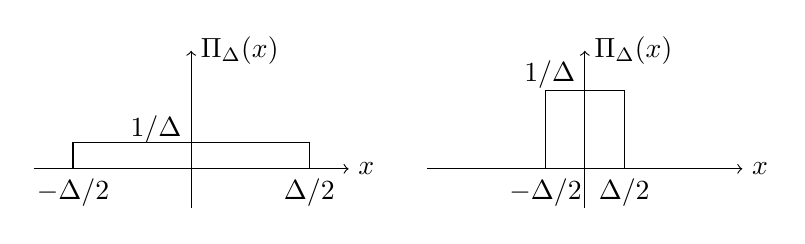
\begin{tikzpicture}
	\begin{scope}
	% Draw the axes
	\draw[->] (-2,0) -- (2,0) node[right] {$x$};
	\draw[->] (0,-0.5) -- (0,1.5) node[right] {$\Pi_\Delta(x)$};
  
  	% Draw the square pulse
  	\def\width{3}
  	\draw (-\width/2,0) -- (-\width/2,1/\width) -- (\width/2,1/\width) -- (\width/2,0);

  	% Add labels (optional)
  	\node[below] at (-\width/2,0) {$-\Delta/2$};
  	\node[below] at (\width/2,0) {$\Delta/2$};
  	\node[left] at (0,1.5/\width) {$1/\Delta$};
	\end{scope}

	\begin{scope}[shift={(5,0)}] % Adjust (5,0) to change the spacing
	% Draw the axes
	\draw[->] (-2,0) -- (2,0) node[right] {$x$};
	\draw[->] (0,-0.5) -- (0,1.5) node[right] {$\Pi_\Delta(x)$};
  
  	% Draw the square pulse
  	\def\width{1}
  	\draw (-\width/2,0) -- (-\width/2,1/\width) -- (\width/2,1/\width) -- (\width/2,0);

  	% Add labels (optional)
  	\node[below] at (-\width/2,0) {$-\Delta/2$};
  	\node[below] at (\width/2,0) {$\Delta/2$};
  	\node[left] at (0,1.2/\width) {$1/\Delta$};
	\end{scope}
  \end{tikzpicture}
 
  In the limit of \(\Delta\) becoming infinitesimal, we can write
    \begin{equation}
		\lim_{\Delta \rightarrow 0} \Pi_\Delta(x)\ =\ \delta(x)
	\end{equation}	
	
	Another definition is through the \textit{Fourier's anti-transform} of a constant function. Thinking of the Fourier domain and its physical meaning, a constant means \textit{energy} at all Fourier frequencies. This corresponds intuitively to a infinitely rapid transition, precisely as the \(\Delta(x)\) is. Then, indicating by \(j\) the imaginary unit, we can write

	\begin{equation}
		\frac{1}{2\pi} \int_{ -\infty}^{ +\infty} e^{ j\ \omega x} d\omega \ =\ \delta(x)
	\end{equation}	

	For more on the generalized functions, as \(\delta(x)\), see \cite{Saichev:2013}.
\end{svgraybox}	




\newpage
\begin{svgraybox}
	{\bf{On \textit{trains} of Dirac's Deltas}}
	\\

	It is easy to express mathematically the juxtaposition of two of more Delta functions, \textit{placed} across distinct points along the same \(x\)-axis. For instance, if these are 5 points, say \(x = - 1\), \(x =	1\), \(x = 2\), \(x = 2.5\), and \(x = 7\), then the resulting function, sketched below
	
	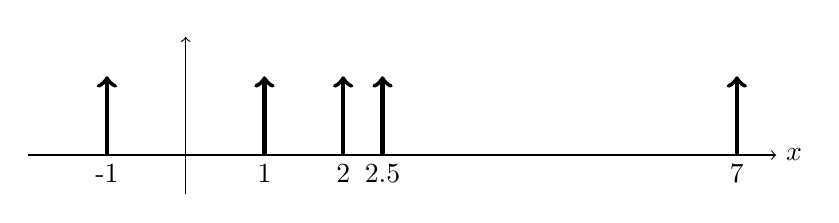
\begin{tikzpicture}
	% Draw the axes
	\draw[->] (-2,0) -- (7.5,0) node[right] {$x$};
	\draw[->] (0,-0.5) -- (0,1.5) node[right] {};
  
	% Draw the Dirac delta function (centered)
	\draw[->, ultra thick] (-1,0) -- (-1,1);
	\draw[->, ultra thick] (1,0) -- (1,1);
	\draw[->, ultra thick] (2,0) -- (2,1);
	\draw[->, ultra thick] (2.5,0) -- (2.5,1);
	\draw[->, ultra thick] (7,0) -- (7,1);
  
	% Add 0 to the origin
	\node[below] at (-1,0) {-1};
	\node[below] at (1,0) {1};
	\node[below] at (2,0) {2};
	\node[below] at (2.5,0) {2.5};
	\node[below] at (7,0) {7};
  \end{tikzpicture}
  
  corresponds mathematically to the algebraic sum of five terms:

  \begin{equation}
	\delta(x + 1)\ +\ \delta(x - 1)\ +\ \delta(x - 2)\ +\ \delta(x - 2.5)\ +\ \delta(x - 7)
  \end{equation}
  
  This is an immediate consequence of the fact that \(\delta(x)\) is zero almost everywhere, so there is absolutely no \textit{interference} or overlap among the \textit{tails} of each term. Note that shifting horizontally to the right (left) the graph of each Dirac's Delta is done subtracting (adding) the appropriate value to the argument of the \(\delta( \bullet )\). A quick way to crosscheck where each Delta is located is searching the value of $x$ that makes its argument zero (e.g., \(x - 2.5 = 0\), only if \(x = 2.5\)).

\end{svgraybox}	
 




\newpage
\begin{svgraybox}
	{\bf{Dirac's Deltas as additive \textit{inputs} to a system}}
	\\
		\begin{center}
		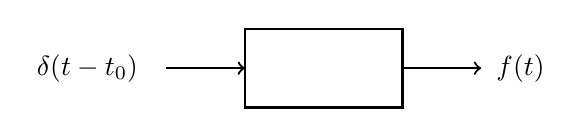
\begin{tikzpicture}		
			% Draw the square
			\draw[thick] (0.,0.5) rectangle (2,1.5);
			
			% Draw the input arrow
			\draw[->, thick] (-1,1) -- (0,1);
			
			% Draw the output arrow
			\draw[->, thick] (2.,1) -- (3,1);
			
			% Add labels
			\node at (-2.,1) {$\delta(t-t_0)$};
			\node at (3.5,1) {$f(t)$};
		\end{tikzpicture}
		\
	\end{center}	
	Consider our \textit{usual} linear o.d.e., say for charge-balance, receptors kinetics, adaptation, synaptic depression, etc. If we \textit{drive} it (e.g., in time) with a Delta, 

	\begin{equation}
		\frac{d}{dt}f(t) = - f(t)\ + \delta(t - t_0),
	\end{equation}

	we can get an analytical solution in two steps. First, we consider the solution \(f(t)\) for times \(t\) far from the occurrence time of the Delta. Before \(t_0\) and after \(t_0\), the Delta vanishes and the o.d.e. becomes homogeneous. In both intervals, the solution looks like an exponential decay \(K\ e^ { - t}\), where \(K\) are constants to be identified. Instead, around \(t_0\) we cannot ignore the impulse, but we can integrate both sides of the equation over an infinitesimal interval \textit{around} \(t_0\):  \(t_0^ -\,  ; t_0^+ \). As we finally invoke linearity of the integral operation, with respect to its argument (i.e., the integral of a sum is the sum of the integrals), we obtain

	\begin{equation}
		\int_{t_0^-}^{t_0^ +} \frac{d}{dt}f(t) dt\ =\ - \int_{t_0^-}^{t_0^ +} f(t) dt\ + \int_{t_0^-}^{t_0^ +} \delta(t - t_0) dt.
	\end{equation}

	The term on the left-hand side is of course the integral of a perfect differential (i.e., integral and derivative signs \textit{cancel out}). From the fundamental theorem of integral calculus~\cite{ThompsonGardner:1998}, we then write it as: \(f(t_0^+) - f(t_0^-)\). Next, the last term on the right-hand side is \(1\), by definition. Finally, as we generally expect the output \(f(t)\) to be \textit{more continuous} than its input \(\delta(t - t_0)\), the remaining term vanishes: it is the integral of a continuous function over an interval of zero length. These considerations brings us to write a simple algebraic additive \textit{update rule}:
	
	\begin{equation}
		f(t_0^+ )\ =\ f(t_0^-)\ +\ 1 
	\end{equation}

	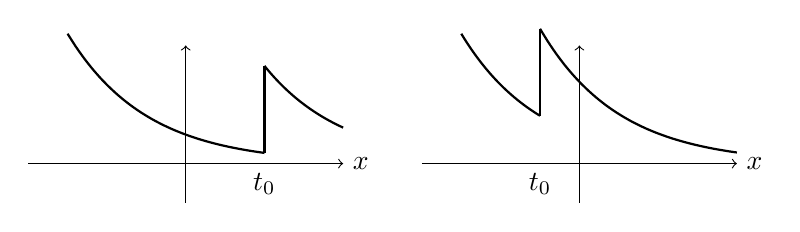
\begin{tikzpicture}
	\begin{scope}
	\draw[->] (-2,0) -- (2.,0) node[right] {$x$};
	\draw[->] (0,-0.5) -- (0,1.5) node[right] {};
  
	% Draw the Dirac delta function (centered)
	\draw[-, thick] (1,{exp(-2)}) -- (1,{exp(.1)+exp(-2)});
	
	% Draw an exponential function decaying from t_0
	\draw[domain=-1.5:1, smooth, variable=\x, thick] plot ({\x}, {exp(-((\x+1)))});
	\draw[domain=1:2, smooth, variable=\x, thick] plot ({\x}, {(exp(.1)+exp(-2))*exp(-((\x-1)))});
  
	% Add 0 to the origin
	\node[below] at (1,0) {$t_0$};
	\end{scope}	% Draw the axes

	\begin{scope}[shift={(5,0)}] % Adjust (5,0) to change the spacing
	\draw[->] (-2,0) -- (2.,0) node[right] {$x$};
	\draw[->] (0,-0.5) -- (0,1.5) node[right] {};
  
	% Draw the Dirac delta function (centered)
	\draw[-, thick] (-0.5,{exp(-0.5)}) -- (-0.5,{exp(.1)+exp(-0.5)});
	
	% Draw an exponential function decaying from t_0
	\draw[domain=-1.5:-0.5, smooth, variable=\x, thick] plot ({\x}, {exp(-((\x+1)))});
	\draw[domain=-0.5:2, smooth, variable=\x, thick] plot ({\x}, {(exp(1.1)+exp(0.5))*exp(-((\x+1.5)))});
  
	% Add 0 to the origin
	\node[below] at (-0.5,0) {$t_0$};
	\end{scope}	% Draw the axes
  \end{tikzpicture}

  Intuitively, an infinite-amplitude input impulse leads to a sudden but finite \textit{jump} in the output, occurring at the time where the impulse occurs. It is then like \textit{adding a fixed quantity} to whatever value \(f(t)\) had immediately before the impulse. Before and after the impulse, the expected decaying exponential dynamics persists.
\end{svgraybox}	
 





\newpage

\begin{svgraybox}
	{\bf{Dirac's Deltas as multiplicative \textit{inputs} to a system}}
	\\

	If the input Delta acts as a multiplicative input, for instance as  

	\begin{equation}
		\frac{d}{dt}f(t) = - f(t)\ +\ f(t) \delta(t - t_0),
	\end{equation}

	we can still get an analytical solution operating in two steps. However, we must now factorize \(f(t)\), separate the variables \(f\) and \(t\), and then integrate over corresponding intervals \textit{around} \(t_0\):  \( (t_0^ -\,  ; t_0^+ ) \) and \( (f_0^ -\,  ; f_0^+ ) \), where \(f_0 = f(t_0)\) if we want to derive some sort of update rule, as in the additive case. 
	
	\begin{equation}
		\int_{f_0^-}^{f_0^+} \frac{df}{f} = \int_{t_0^ -}^{t_0^+} (\delta(t - t_0) - 1)dt.
	\end{equation}

	The left hand side is solved, recalling that the primitive of \(1/x\) is \(\ln(x)\). We can also use the property that a difference of logs equals the log of the ratio. So we write 

	\begin{equation}
		\ln \frac{f(t_0^+)}{f_(t_0^-)} = 1,
	\end{equation}

	where the right-hand side contains only the term \(1 \) corresponding to the area of the Dirac's Delta, as the other term (i.e., the integral of \( -1\) over an interval of zero length) vanished. We then apply the exponential to both sides, making \(f\) explicit and leading to a multiplicative algebraic \textit{update rule}:
	
	\begin{equation}
		f(t_0^+)\ =\ e^{1} f(t_0^-)
	\end{equation}

	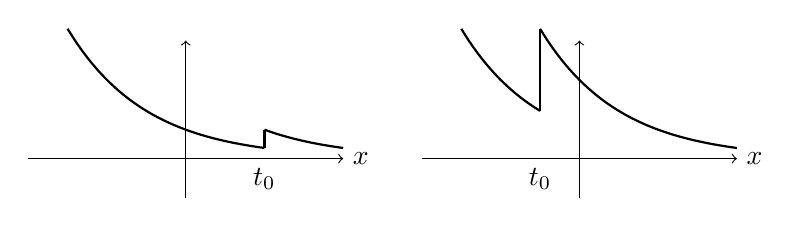
\begin{tikzpicture}
	\begin{scope}
	\draw[->] (-2,0) -- (2.,0) node[right] {$x$};
	\draw[->] (0,-0.5) -- (0,1.5) node[right] {};
  
	% Draw the Dirac delta function (centered)
	\draw[-, thick] (1,{exp(-2)}) -- (1,{exp(1)*exp(-2)});
	
	% Draw an exponential function decaying from t_0
	\draw[domain=-1.5:1, smooth, variable=\x, thick] plot ({\x}, {exp(-((\x+1)))});
	\draw[domain=1:2, smooth, variable=\x, thick] plot ({\x}, {(exp(1)*exp(-2))*exp(-((\x-1)))});
  
	% Add 0 to the origin
	\node[below] at (1,0) {$t_0$};
	\end{scope}	% Draw the axes

	\begin{scope}[shift={(5,0)}] % Adjust (5,0) to change the spacing
	\draw[->] (-2,0) -- (2.,0) node[right] {$x$};
	\draw[->] (0,-0.5) -- (0,1.5) node[right] {};
  
	% Draw the Dirac delta function (centered)
	\draw[-, thick] (-0.5,{exp(-0.5)}) -- (-0.5,{exp(1)*exp(-0.5)});
	
	% Draw an exponential function decaying from t_0
	\draw[domain=-1.5:-0.5, smooth, variable=\x, thick] plot ({\x}, {exp(-((\x+1)))});
	\draw[domain=-0.5:2, smooth, variable=\x, thick] plot ({\x}, {(exp(1)*exp(0.5))*exp(-((\x+1.5)))});
  
	% Add 0 to the origin
	\node[below] at (-0.5,0) {$t_0$};
	\end{scope}	% Draw the axes
  \end{tikzpicture}

  Intuitively, an infinite-amplitude (multiplicative) input impulse leads to a \textit{jump} in the output, but the size of this jump is proportional to the value of \(f(t)\) immediately before the impulse. Before and after the impulse, the expected decaying exponential dynamics persists.
\end{svgraybox}	
 








\begin{thebibliography}{99.}%
% Contribution 
\bibitem{science-contrib} Broy, M.: Software engineering --- from auxiliary to key technologies. In: Broy, M., Dener, E. (eds.) Software Pioneers, pp. 10-13. Springer, Heidelberg (2002)
%
% Online Document
\bibitem{science-online} Dod, J.: Effective substances. In: The Dictionary of Substances and Their Effects. Royal Society of Chemistry (1999) Available via DIALOG. \\
\url{http://www.rsc.org/dose/title of subordinate document. Cited 15 Jan 1999}
%
% Monograph
\bibitem{Saichev:2013} Saichev, A.I., Woyczy, W.A.: Distributions in the Physical and Engineering Sciences. Vol. 2, Appendix C, Birkhäuser-Boston (2013) 

\bibitem{ThompsonGardner:1998} Thompson, S., Gardner, M.: Calculus Made Easy. 2nd ed., St. Martin's Press (1998) 
%
\bibitem{science-mono} Geddes, K.O., Czapor, S.R., Labahn, G.: Algorithms for Computer Algebra. Kluwer, Boston (1992) 
%
% Journal article
\bibitem{science-journal} Hamburger, C.: Quasimonotonicity, regularity and duality for nonlinear systems of partial differential equations. Ann. Mat. Pura. Appl. \textbf{169}, 321--354 (1995)
%
% Journal article by DOI
\bibitem{science-DOI} Slifka, M.K., Whitton, J.L.: Clinical implications of dysregulated cytokine production. J. Mol. Med. (2000) doi: 10.1007/s001090000086 

\end{thebibliography}